% ============================================================
%  SECCIÓN 2 – DESCRIPCIÓN DE LA HERRAMIENTA DE SOFTWARE
% ============================================================
\section{Descripción de la Herramienta de Software}

\subsection{Definición General}

!Blood es una aplicación móvil orientada a la donación de sangre que permite a cualquier persona integrarse a una comunidad de apoyo, con la posibilidad de donar o solicitar sangre según la necesidad. La herramienta centraliza solicitudes, campañas y comunicación entre usuarios, priorizando la compatibilidad por tipo de sangre y la cercanía geográfica, para facilitar respuestas oportunas.

La aplicación contempla dos perfiles de usuario diferenciados ---ciudadano y profesional de salud--- y estructura su funcionamiento en torno a módulos claramente definidos que cubren desde el registro y verificación de identidad hasta la gestión de campañas institucionales.

% ──────────────────────────────────────────────────────────
\subsection{Arquitectura Funcional}

A continuación se describen en detalle los módulos funcionales que componen la aplicación, organizados según el flujo natural de interacción del usuario.

% ── 2.2.1 ─────────────────────────────────────────────────
\subsubsection{Pantalla de Bienvenida (Splash)}

La pantalla de bienvenida constituye el primer punto de contacto del usuario con la aplicación. Presenta la identidad visual de !Blood ---logotipo con la gota de sangre y el eslogan ``Dona vida, recibe vida''--- acompañada de un mensaje de comunidad: \textit{``Juntos creamos una comunidad que salva vidas''}. Desde esta pantalla, el usuario accede a dos acciones principales:

\begin{itemize}
    \item \textbf{Iniciar Sesión:} redirige a la pantalla de autenticación para usuarios ya registrados.
    \item \textbf{Registrarme:} inicia el flujo de creación de cuenta en tres pasos.
\end{itemize}

La interfaz de bienvenida se ilustra en la Figura~\ref{fig:splash}.

\begin{figure}[H]
  \centering
  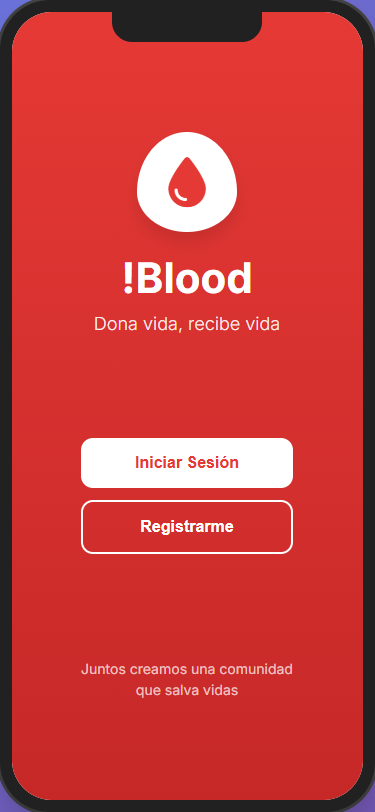
\includegraphics[width=0.32\textwidth]{imagenes/01_splash.png}
  \caption{Pantalla de bienvenida (Splash).}
  \label{fig:splash}
\end{figure}

% ── 2.2.2 ─────────────────────────────────────────────────
\subsubsection{Inicio de Sesión (Login)}

El módulo de inicio de sesión permite al usuario autenticarse mediante su correo electrónico o nombre de usuario y su contraseña. La interfaz incluye:

\begin{itemize}
    \item Campo de usuario o correo electrónico con icono contextual.
    \item Campo de contraseña con opción de alternar la visibilidad del texto ingresado (botón de ojo).
    \item Enlace de recuperación de contraseña (\textit{``¿Olvidaste tu contraseña?''}).
    \item Enlace de acceso rápido al registro para usuarios nuevos.
\end{itemize}

El diseño prioriza la simplicidad: formulario limpio, botones claros y retroalimentación visual inmediata, como se aprecia en la Figura~\ref{fig:login}.

\begin{figure}[H]
  \centering
  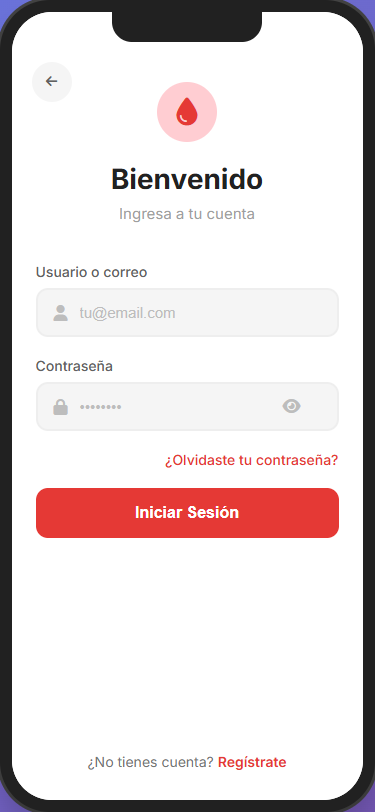
\includegraphics[width=0.32\textwidth]{imagenes/02_login.png}
  \caption{Pantalla de inicio de sesión.}
  \label{fig:login}
\end{figure}

% ── 2.2.3 ─────────────────────────────────────────────────
\subsubsection{Registro de Usuario}

El proceso de registro se estructura en tres pasos secuenciales, con un indicador de progreso visible que informa al usuario en qué etapa se encuentra (véase Figura~\ref{fig:registro}).

\paragraph{Paso 1: Datos Personales.}
En esta primera etapa, el usuario proporciona:

\begin{itemize}
    \item \textbf{Tipo de usuario:} selección entre \textit{Ciudadano} o \textit{Profesional de salud}. Esta distinción habilita funcionalidades diferenciadas (por ejemplo, la creación de campañas está reservada al perfil profesional).
    \item \textbf{Nombre completo.}
    \item \textbf{Fecha de nacimiento.}
    \item \textbf{Tipo de sangre:} selección entre los ocho grupos sanguíneos (A+, A-, B+, B-, AB+, AB-, O+, O-).
    \item \textbf{Cédula de ciudadanía.}
    \item \textbf{Teléfono de contacto.}
    \item \textbf{Correo electrónico.}
\end{itemize}

\paragraph{Paso 2: Verificación.}
La segunda etapa tiene como objetivo validar la identidad del usuario y registrar su ubicación:

\begin{itemize}
    \item \textbf{Fotografía de la cédula de ciudadanía:} el usuario carga una imagen legible de su documento de identidad.
    \item \textbf{Foto de perfil:} se solicita una fotografía con fondo blanco y rostro visible, para facilitar la identificación entre usuarios.
    \item \textbf{Ciudad de residencia.}
    \item \textbf{Dirección:} campo de texto complementado con un botón de geolocalización automática que permite capturar la ubicación actual del dispositivo.
\end{itemize}

\paragraph{Paso 3: Configuración de Cuenta.}
En la última etapa del registro se configuran las credenciales de acceso:

\begin{itemize}
    \item \textbf{Nombre de usuario:} identificador único dentro de la plataforma.
    \item \textbf{Contraseña:} con indicador visual de fortaleza (baja, media, alta) que orienta al usuario a crear una contraseña segura.
    \item \textbf{Confirmación de contraseña.}
    \item \textbf{Aceptación de términos y condiciones} y de la política de privacidad.
    \item \textbf{Compromiso de donación solidaria:} el usuario acepta explícitamente que toda donación canalizada a través de la plataforma es voluntaria y sin fines de lucro.
\end{itemize}

\begin{figure}[H]
  \centering
  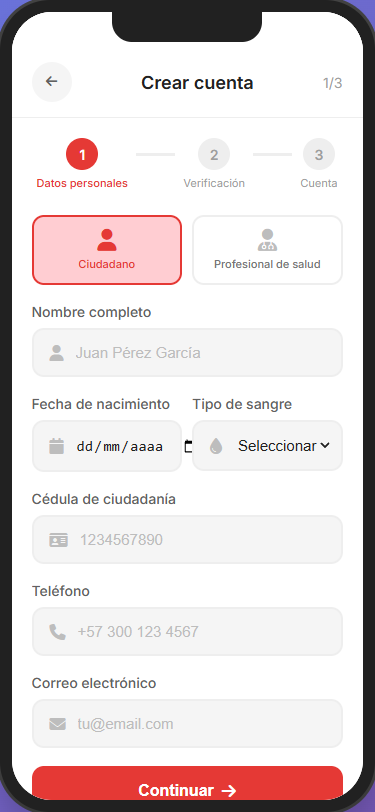
\includegraphics[width=0.32\textwidth]{imagenes/03_registro_paso1.png}\hfill
  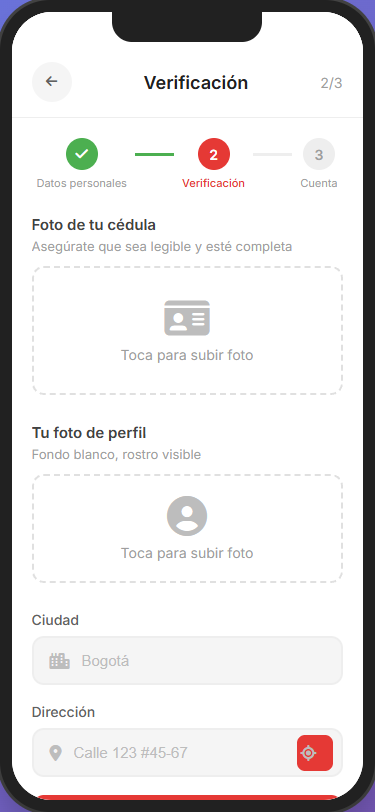
\includegraphics[width=0.32\textwidth]{imagenes/04_registro_paso2.png}\hfill
  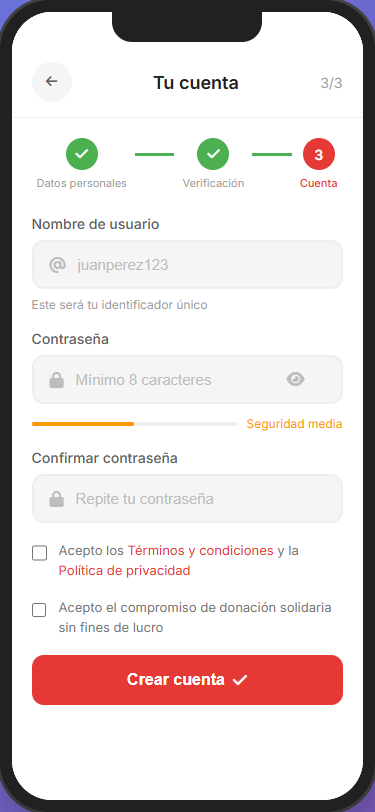
\includegraphics[width=0.32\textwidth]{imagenes/05_registro_paso3.png}
  \caption{Flujo de registro en tres pasos: datos personales (izq.), verificación de identidad (centro) y configuración de cuenta (der.).}
  \label{fig:registro}
\end{figure}

% ── 2.2.4 ─────────────────────────────────────────────────
\subsubsection{Pantalla Principal (Home)}

La pantalla principal es el centro de operaciones del usuario tras iniciar sesión. Está compuesta por los siguientes elementos:

\paragraph{Encabezado personalizado.}
Muestra el avatar, el saludo personalizado con el nombre del usuario y un botón de acceso directo a las notificaciones, con indicador numérico de notificaciones pendientes.

\paragraph{Tarjeta de sangre del usuario.}
Panel destacado que presenta el tipo de sangre del usuario junto con sus estadísticas de participación: número de donaciones realizadas y vidas ayudadas. Este elemento refuerza la motivación y el sentido de impacto.

\paragraph{Acciones rápidas.}
Cuadrícula de cuatro accesos directos a las funcionalidades principales:

\begin{itemize}
    \item \textbf{Solicitar sangre:} abre el formulario de creación de solicitud.
    \item \textbf{Ver solicitudes:} accede al listado de solicitudes activas en la zona.
    \item \textbf{Campañas:} muestra las campañas de donación programadas.
    \item \textbf{Mensajes:} dirige al módulo de chat.
\end{itemize}

\paragraph{Solicitudes cercanas.}
Listado resumido de las solicitudes de sangre activas más próximas al usuario, mostrando para cada una: nombre del solicitante, tipo de sangre requerido, distancia en kilómetros y tiempo transcurrido desde la publicación.

\paragraph{Campañas próximas.}
Vista previa de las campañas de donación programadas en la zona, con información de la institución organizadora, fecha, hora y distancia.

\paragraph{Estadísticas de comunidad.}
Indicadores globales que muestran el total de donantes activos y vidas salvadas en la plataforma, reforzando el sentido de pertenencia a una comunidad con impacto real.

\paragraph{Barra de navegación inferior.}
Barra fija con cinco elementos: Inicio, Explorar, botón central prominente de creación rápida (+), Chat y Perfil. El botón central se destaca visualmente como un botón de acción flotante (FAB). La composición completa de la pantalla principal se puede observar en la Figura~\ref{fig:home}.

\begin{figure}[H]
  \centering
  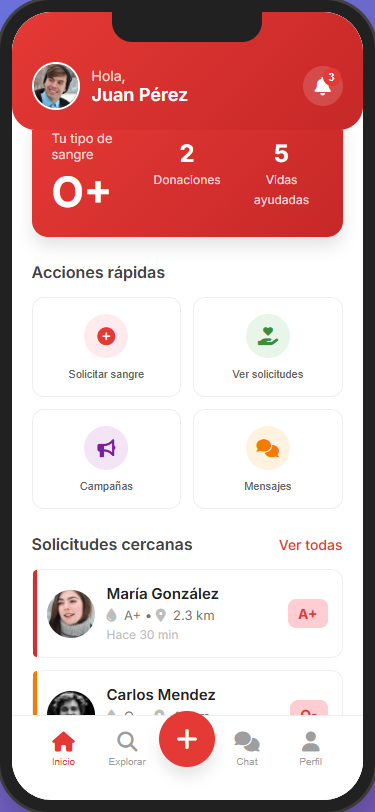
\includegraphics[width=0.32\textwidth]{imagenes/06_home.png}
  \caption{Pantalla principal (Home) con tarjeta de tipo de sangre, acciones rápidas y solicitudes cercanas.}
  \label{fig:home}
\end{figure}

% ── 2.2.5 ─────────────────────────────────────────────────
\subsubsection{Creación de Solicitud de Sangre}

Este módulo permite a cualquier usuario publicar una solicitud de sangre. El formulario recoge:

\begin{itemize}
    \item \textbf{Tipo de sangre necesario:} selector visual con los ocho grupos sanguíneos.
    \item \textbf{Unidades necesarias:} control numérico con botones de incremento y decremento (rango de 1 a 10 unidades).
    \item \textbf{Nivel de urgencia:} tres opciones diferenciadas por color e iconografía:
    \begin{itemize}
        \item \textit{Bajo:} puede esperar días.
        \item \textit{Medio:} se necesita en las próximas horas.
        \item \textit{Urgente:} se necesita lo antes posible.
    \end{itemize}
    \item \textbf{Centro de salud:} selección del centro médico donde se realizará la donación.
    \item \textbf{Mensaje para donantes:} campo de texto opcional (máximo 200 caracteres).
\end{itemize}

Un banner informativo aclara: \textit{``Tu solicitud será visible para donantes compatibles en tu zona''}. Tras enviar la solicitud, se muestra una pantalla de confirmación que informa el número de donantes notificados. El formulario y la confirmación se ilustran en la Figura~\ref{fig:crear-solicitud}.

\begin{figure}[H]
  \centering
  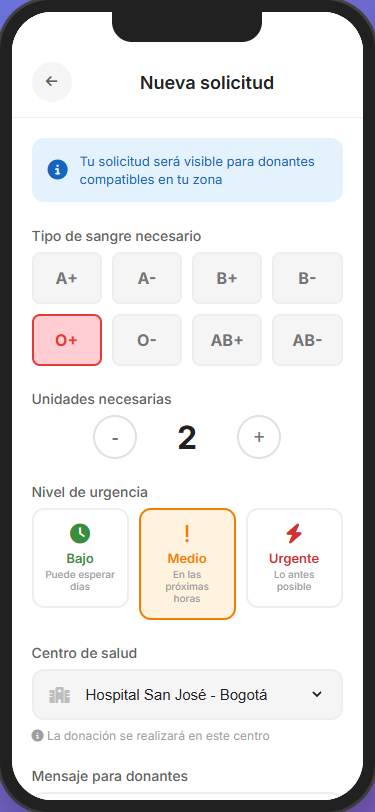
\includegraphics[width=0.32\textwidth]{imagenes/07_crear_solicitud.png}\hfill
  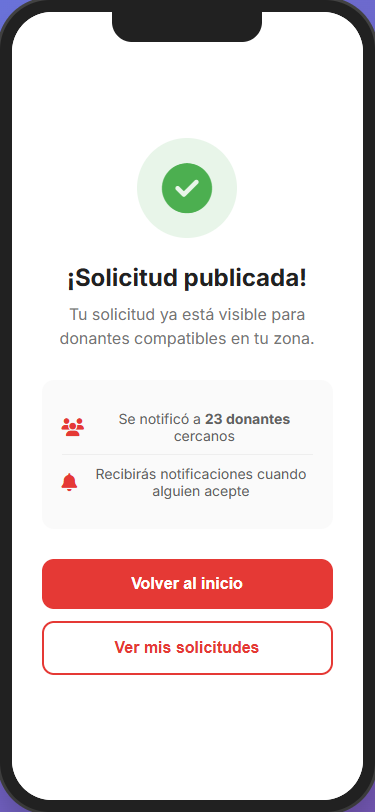
\includegraphics[width=0.32\textwidth]{imagenes/08_solicitud_exitosa.png}
  \caption{Formulario de creación de solicitud (izq.) y confirmación de publicación (der.).}
  \label{fig:crear-solicitud}
\end{figure}

% ── 2.2.6 ─────────────────────────────────────────────────
\subsubsection{Exploración de Solicitudes}

La pantalla de solicitudes presenta el listado completo de solicitudes activas en la zona. Incluye:

\begin{itemize}
    \item \textbf{Barra de búsqueda:} por nombre del solicitante o tipo de sangre.
    \item \textbf{Filtros rápidos (chips):} Todas, Urgentes, Compatible y Cercanas.
\end{itemize}

Cada tarjeta muestra: nivel de urgencia, tiempo de publicación, solicitante, tipo de sangre, unidades, centro de salud, distancia y mensaje breve, tal como se aprecia en la Figura~\ref{fig:solicitudes}.

\begin{figure}[H]
  \centering
  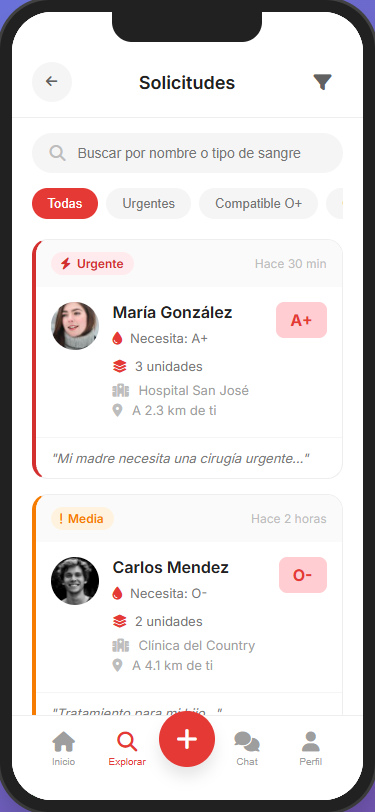
\includegraphics[width=0.32\textwidth]{imagenes/09_solicitudes.png}
  \caption{Listado de solicitudes activas con filtros y búsqueda.}
  \label{fig:solicitudes}
\end{figure}

% ── 2.2.7 ─────────────────────────────────────────────────
\subsubsection{Detalle de Solicitud}

Vista completa de una solicitud que comprende:

\begin{itemize}
    \item Encabezado con urgencia, tipo de sangre y unidades.
    \item Información del solicitante con sello de verificación.
    \item Mensaje completo de la situación.
    \item Centro de salud con dirección, distancia y botón de mapa.
    \item Estado de donantes aceptados respecto al total requerido.
    \item \textbf{Aviso de compatibilidad automática:} el sistema informa si el tipo de sangre del usuario es compatible.
    \item Botón \textit{``Quiero donar''} que conduce al flujo de confirmación.
    \item Nota que aclara que la comunicación posterior se realiza vía chat interno y que la donación ocurre únicamente en el centro de salud indicado.
\end{itemize}

La vista completa del detalle de solicitud se muestra en la Figura~\ref{fig:detalle-solicitud}.

\begin{figure}[H]
  \centering
  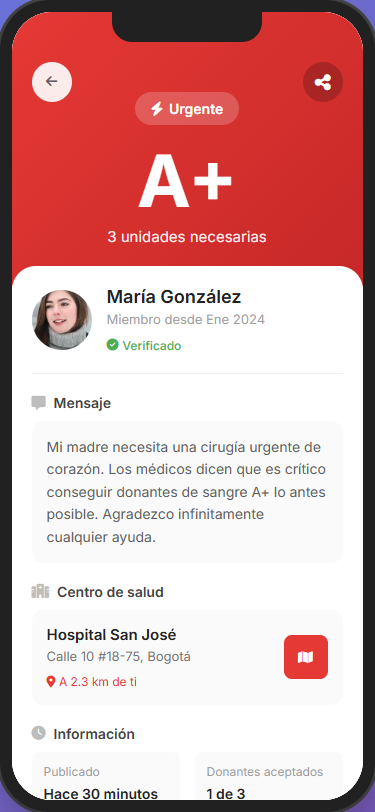
\includegraphics[width=0.32\textwidth]{imagenes/10_detalle_solicitud.png}
  \caption{Vista detallada de una solicitud: urgencia, datos del solicitante, compatibilidad y botón de donación.}
  \label{fig:detalle-solicitud}
\end{figure}

% ── 2.2.8 ─────────────────────────────────────────────────
\subsubsection{Confirmación de Donación}

Antes de confirmar, el usuario revisa un resumen y acepta:

\begin{itemize}
    \item \textbf{Compromiso del donante:} acudir al centro indicado, donación voluntaria y sin fines de lucro, comunicación limitada a la coordinación.
    \item \textbf{Checklist de salud:} no haber donado en los últimos 3 meses, ausencia de enfermedades infectocontagiosas, edad entre 18 y 65 años, peso mayor a 50\,kg.
\end{itemize}

Al confirmar, una pantalla de agradecimiento reconoce al donante e indica el centro de salud al que debe acudir. Ambas pantallas se ilustran en la Figura~\ref{fig:confirmar-donacion}.

\begin{figure}[H]
  \centering
  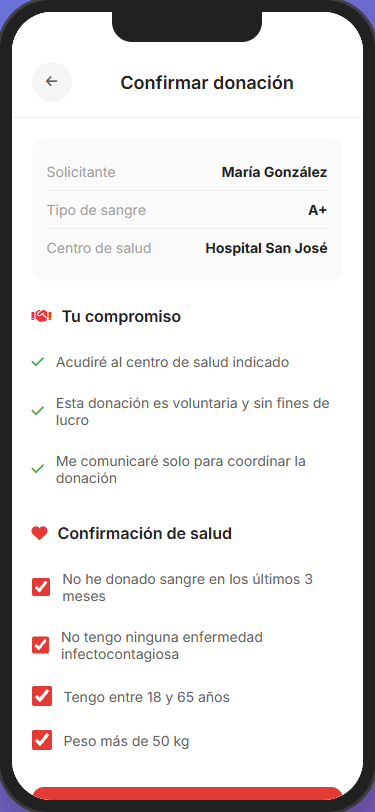
\includegraphics[width=0.32\textwidth]{imagenes/11_confirmar_donacion.png}\hfill
  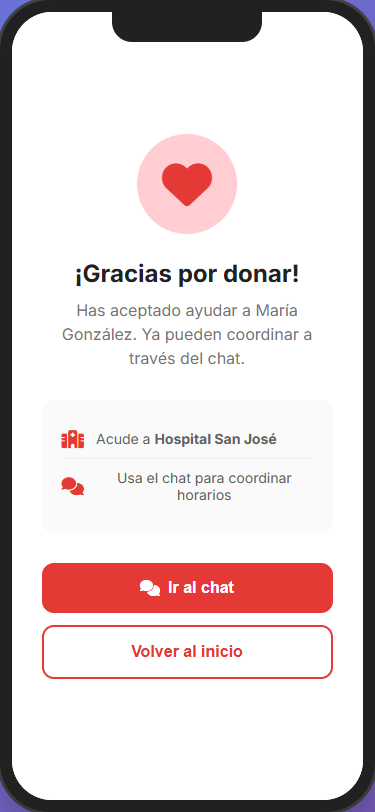
\includegraphics[width=0.32\textwidth]{imagenes/12_donacion_confirmada.png}
  \caption{Resumen de compromiso y checklist de salud previo a la donación (izq.) y pantalla de agradecimiento al donante (der.).}
  \label{fig:confirmar-donacion}
\end{figure}

% ── 2.2.9 ─────────────────────────────────────────────────
\subsubsection{Sistema de Mensajería (Chat)}

El módulo de mensajería activa la comunicación directa entre donante y solicitante, exclusivamente en el contexto de una donación aceptada.

\paragraph{Lista de conversaciones.}
Muestra todas las conversaciones activas con: foto del interlocutor, estado en línea, nombre, última hora de actividad, vista previa del último mensaje, indicador de no leídos y contexto de la solicitud asociada (tipo de sangre y estado).

\paragraph{Detalle de conversación.}
Incluye encabezado con datos del interlocutor y solicitud, burbujas de mensajes diferenciadas (enviados/recibidos), marcas de tiempo, indicadores de lectura (doble check) y separadores de fecha. El elemento destacado es el \textbf{aviso de moderación por IA}: banner visible que informa \textit{``Chat protegido por IA -- Solo mensajes relacionados con la donación''}, filtrando automáticamente contenido inadecuado o no relacionado con el propósito de la plataforma. La lista de conversaciones y el chat activo se muestran en la Figura~\ref{fig:chat}.

\begin{figure}[H]
  \centering
  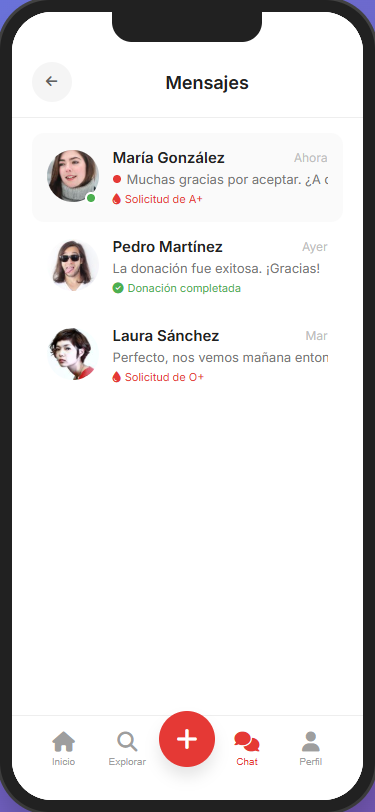
\includegraphics[width=0.32\textwidth]{imagenes/13_chat_lista.png}\hfill
  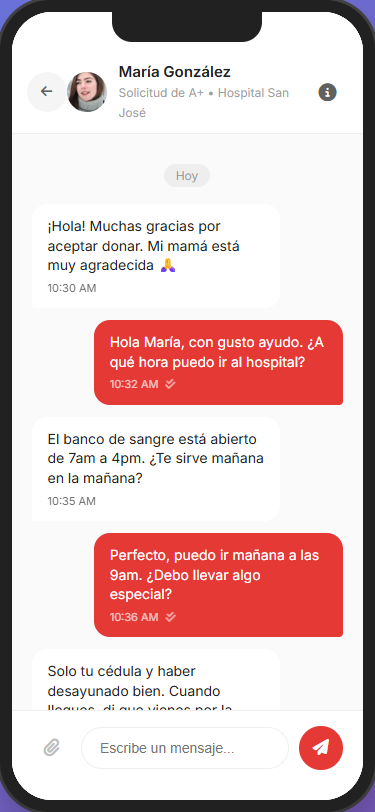
\includegraphics[width=0.32\textwidth]{imagenes/14_chat_detalle.png}
  \caption{Lista de conversaciones con contexto de solicitud (izq.) y chat de coordinación con aviso de moderación por IA (der.).}
  \label{fig:chat}
\end{figure}

% ── 2.2.10 ────────────────────────────────────────────────
\subsubsection{Perfil de Usuario}

La pantalla de perfil concentra la información personal y la configuración:

\begin{itemize}
    \item Foto de perfil editable, nombre y nombre de usuario.
    \item Insignias de \textit{Verificado} y \textit{Donante activo}.
    \item Tarjeta con tipo de sangre, donaciones realizadas, vidas ayudadas y solicitudes creadas.
    \item Datos de contacto y antigüedad.
    \item Accesos a: editar perfil, notificaciones, privacidad, ayuda y cerrar sesión.
\end{itemize}

La pantalla de perfil se ilustra en la Figura~\ref{fig:perfil}.

\begin{figure}[H]
  \centering
  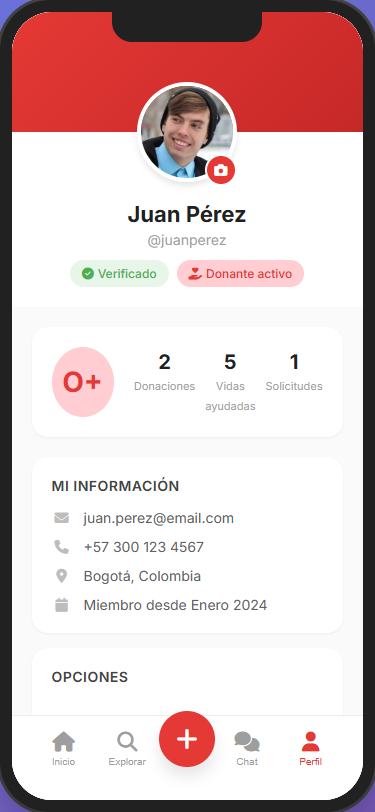
\includegraphics[width=0.32\textwidth]{imagenes/15_perfil.png}
  \caption{Perfil de usuario: insignias de verificación, estadísticas de donación y opciones de configuración.}
  \label{fig:perfil}
\end{figure}

% ── 2.2.11 ────────────────────────────────────────────────
\subsubsection{Sistema de Notificaciones}

Mantiene al usuario informado en tiempo real. Tipos de notificación:

\begin{itemize}
    \item \textbf{Solicitudes urgentes:} alerta cuando hay sangre compatible y cercana disponible.
    \item \textbf{Mensajes nuevos:} aviso de chat entrante.
    \item \textbf{Donaciones confirmadas:} registro exitoso de una donación.
    \item \textbf{Reconocimientos:} mensajes motivacionales por logros alcanzados.
    \item \textbf{Estadísticas de comunidad:} crecimiento de la plataforma.
\end{itemize}

Las notificaciones se distinguen visualmente entre leídas y no leídas, con opción global de marcar todas como leídas, como se aprecia en la Figura~\ref{fig:notificaciones}.

\begin{figure}[H]
  \centering
  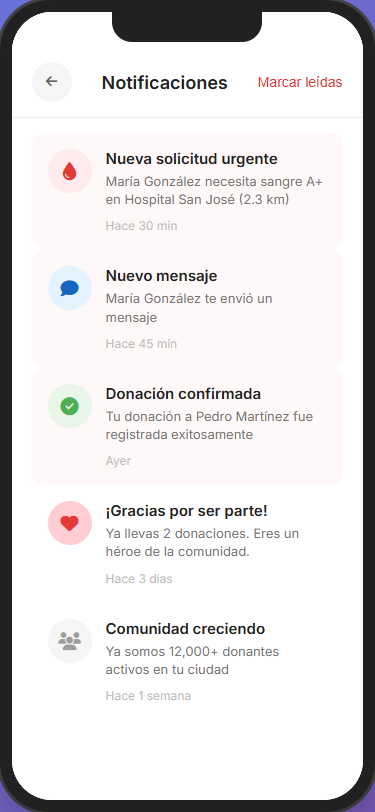
\includegraphics[width=0.32\textwidth]{imagenes/16_notificaciones.png}
  \caption{Centro de notificaciones: solicitudes urgentes, mensajes, confirmaciones y reconocimientos.}
  \label{fig:notificaciones}
\end{figure}

% ── 2.2.12 ────────────────────────────────────────────────
\subsubsection{Gestión de Solicitudes Propias}

El usuario puede revisar sus solicitudes organizadas en pestañas: \textit{Activas}, \textit{Completadas} y \textit{Canceladas}. Para cada solicitud activa se muestra: tipo de sangre, centro, fecha de creación, barra de progreso de donantes confirmados, avatares de donantes y botones de acción (\textit{Ver detalles} / \textit{Cancelar}), tal como se observa en la Figura~\ref{fig:mis-solicitudes}.

\begin{figure}[H]
  \centering
  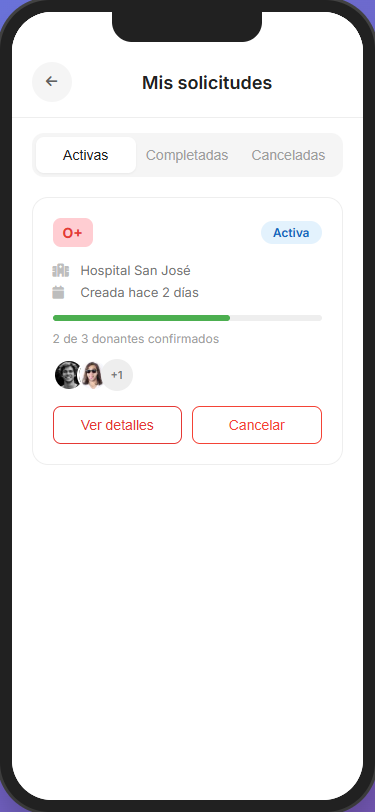
\includegraphics[width=0.32\textwidth]{imagenes/17_mis_solicitudes.png}
  \caption{Gestión de solicitudes propias: progreso de donantes confirmados y acciones disponibles.}
  \label{fig:mis-solicitudes}
\end{figure}

% ── 2.2.13 Campañas ───────────────────────────────────────
\subsubsection{Campañas de Donación}

Las campañas son una funcionalidad exclusiva para usuarios con perfil de \textbf{profesional de salud}, que permite a las instituciones organizar y promocionar jornadas masivas de donación.

\paragraph{Creación de campaña.}
El formulario recoge:

\begin{itemize}
    \item Nombre de la campaña.
    \item Centro de salud o institución organizadora.
    \item Dirección del evento con soporte de geolocalización.
    \item Fecha, hora de inicio y hora de finalización.
    \item Cupos disponibles.
    \item Tipos de sangre necesarios (selección múltiple o ``Todos'').
    \item Descripción de la campaña (máximo 500 caracteres): objetivos, beneficios para donantes, información relevante.
    \item Requisitos estandarizados: edad 18--65 años, peso $> 50$\,kg, documento de identidad, mínimo 3 meses desde la última donación.
    \item Teléfono de contacto.
\end{itemize}

El formulario de creación y la pantalla de confirmación se muestran en la Figura~\ref{fig:crear-campana}.

\begin{figure}[H]
  \centering
  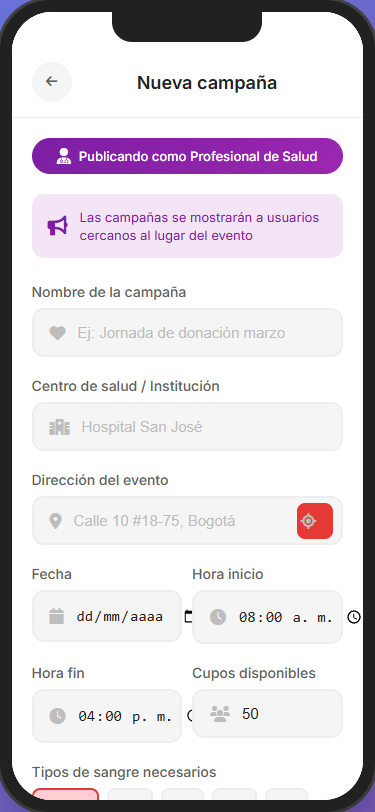
\includegraphics[width=0.32\textwidth]{imagenes/18_crear_campana.png}\hfill
  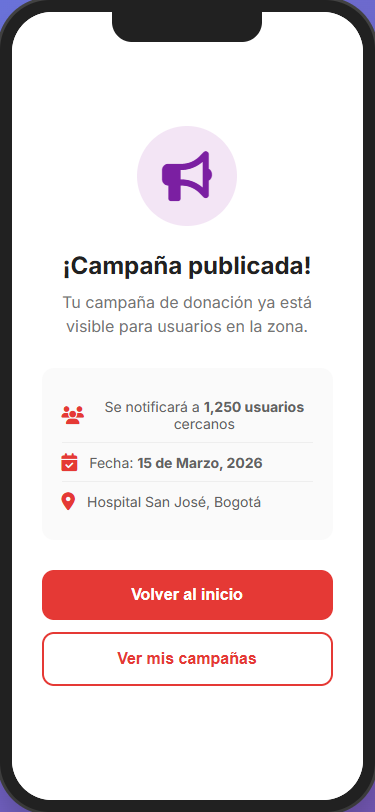
\includegraphics[width=0.32\textwidth]{imagenes/19_campana_exitosa.png}
  \caption{Formulario de creación de campaña con campos de horario y tipos de sangre (izq.) y confirmación de publicación con alcance estimado (der.).}
  \label{fig:crear-campana}
\end{figure}

\paragraph{Exploración de campañas.}
Todos los usuarios pueden consultar las campañas disponibles con barra de búsqueda, filtros (Cercanas, Esta semana, Este mes) y tarjetas que muestran: fecha, institución, dirección, horario, distancia y disponibilidad de cupos.

\paragraph{Detalle de campaña.}
La vista completa incluye: organización verificada, descripción, mapa de ubicación, horario, tipos de sangre con indicación de los más urgentes, requisitos, indicador de cupos (reservados/disponibles con barra de progreso), contacto y botón de \textit{``Reservar mi cupo''}. El listado y el detalle se ilustran en la Figura~\ref{fig:campanas}.

\begin{figure}[H]
  \centering
  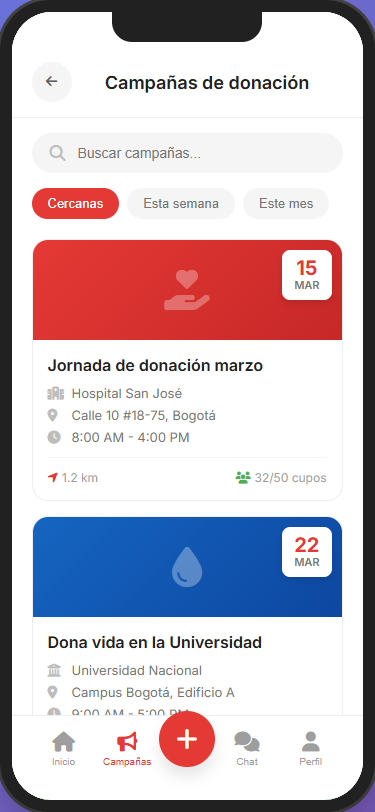
\includegraphics[width=0.32\textwidth]{imagenes/20_campanas.png}\hfill
  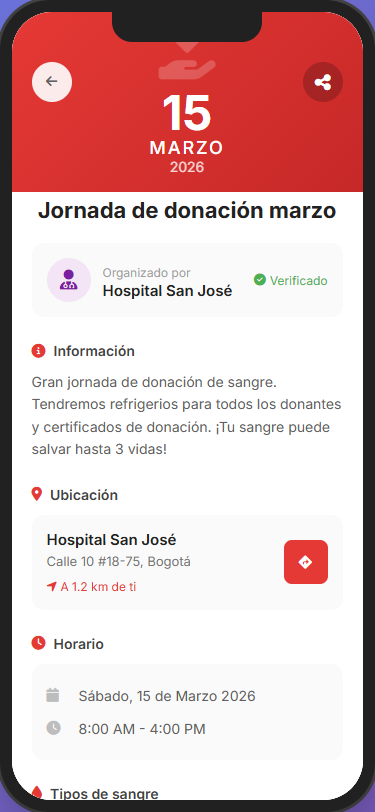
\includegraphics[width=0.32\textwidth]{imagenes/21_detalle_campana.png}
  \caption{Listado de campañas con fecha, institución y cupos disponibles (izq.) y vista detallada con horario, tipos de sangre y opción de reserva (der.).}
  \label{fig:campanas}
\end{figure}

% ──────────────────────────────────────────────────────────
\subsection{Características Transversales}

\begin{itemize}
    \item \textbf{Compatibilidad inteligente:} el sistema evalúa automáticamente la compatibilidad entre el tipo de sangre del donante y el requerido.
    \item \textbf{Geolocalización:} todas las solicitudes y campañas muestran distancia respecto al usuario.
    \item \textbf{Verificación de identidad:} el registro requiere cédula y fotografía, generando un sello de \textit{Verificado} que otorga confianza.
    \item \textbf{Moderación por inteligencia artificial:} el chat incorpora filtrado automático para garantizar que la comunicación se limite al contexto de la donación.
    \item \textbf{Modelo solidario:} la plataforma refuerza en cada flujo que las donaciones son voluntarias y sin fines de lucro.
    \item \textbf{Gamificación y reconocimiento:} estadísticas, insignias y mensajes motivacionales fomentan la participación recurrente.
    \item \textbf{Interfaz inclusiva:} diseño con tipografía clara, iconografía intuitiva, campos con pistas contextuales y flujos cortos que minimizan la carga cognitiva.
\end{itemize}
